\documentclass[12pt]{article}

% ==============================================================================
% SMARTHEALTH IOT — SYSTEM WORKFLOW & TECHNICAL SPECIFICATION REPORT
% Department of Electronics and Communication Engineering
% Cooch Behar Government Engineering College (CGEC)
% Affiliated to Maulana Abul Kalam Azad University of Technology (MAKAUT), West Bengal
% Strict Black & White (Monochrome) Master Specification
% Body Font: Calibri | Dynamic Heading Scale per biraj-xelatex-general-specs.md
% Preserved File Name: SmartHealth_IoT_Workflow_Report.tex
% ==============================================================================

\usepackage[a4paper, margin=0.8in, headheight=0pt, headsep=12pt, footskip=22pt]{geometry}
\usepackage{fontspec}
\usepackage{unicode-math}

% --- Typography (Calibri Body per User Specification) ---
\setmainfont{Calibri}
\setsansfont{Calibri}
\setmonofont{Consolas}
\setmathfont{Cambria Math}

\usepackage{setspace}
\setstretch{1.18}
\setlength{\parindent}{0pt}
\setlength{\parskip}{4pt}
\hyphenpenalty=10000
\exhyphenpenalty=10000
\raggedright
\raggedbottom

% --- Core Packages ---
\usepackage{graphicx}
\usepackage{xcolor}
\usepackage{amsmath}
\usepackage{array}
\usepackage{enumitem}
\usepackage{float}
\renewcommand{\topfraction}{0.95}
\renewcommand{\bottomfraction}{0.95}
\renewcommand{\textfraction}{0.05}
\renewcommand{\floatpagefraction}{0.9}
\usepackage{fancyhdr}
\usepackage{lastpage}
\usepackage{titlesec}
\usepackage{tcolorbox}
\tcbuselibrary{skins}

% --- TikZ Vector Diagramming (B/W Mode) ---
\usepackage{tikz}
\usetikzlibrary{arrows.meta, positioning, calc, shapes.geometric, fit, backgrounds}

% --- Hyperlinks Configuration (Monochrome / Clean Black in B/W Mode) ---
\usepackage[colorlinks=true, linkcolor=black, urlcolor=black, citecolor=black, linktoc=all, bookmarksnumbered=true]{hyperref}

% --- Running Headers & Footers (No Header Text, No Footer HRule Separator) ---
\pagestyle{fancy}
\fancyhf{}
\renewcommand{\headrulewidth}{0pt}
\renewcommand{\footrulewidth}{0pt}
\fancyfoot[C]{\small\thepage\ of \pageref{LastPage}}

% --- Heading Typography per biraj-xelatex-general-specs.md ---
% Depth: Top-level (\section) + 1 Sub-level (\subsection)
% Body: 12pt regular
% Sub-level: 14pt bold (12 + 2)
% Top-level: 17pt bold, centered, all CAPS, and underlined (User requirement)
\newcommand{\titleunderline}[1]{\underline{\thesection.\ \MakeUppercase{#1}}}
\titleformat{\section}[block]
  {\fontsize{17}{22}\selectfont\bfseries\centering\color{black}}
  {}{0pt}{\titleunderline}

\newcommand{\titleunderlinenumless}[1]{\underline{\MakeUppercase{#1}}}
\titleformat{name=\section,numberless}[block]
  {\fontsize{17}{22}\selectfont\bfseries\centering\color{black}}
  {}{0pt}{\titleunderlinenumless}

\titlespacing*{\section}{0pt}{10pt}{6pt}

\titleformat{\subsection}
  {\fontsize{14}{17}\selectfont\bfseries\color{black}}
  {\thesubsection}{0.5em}{}
\titlespacing*{\subsection}{0pt}{7pt}{2pt}

% --- Table Column Specifications & Width Budgeting ---
\newcolumntype{L}[1]{>{\raggedright\arraybackslash}m{#1}}
\newcolumntype{B}[1]{>{\raggedright\arraybackslash\bfseries}m{#1}}
\newcolumntype{C}[1]{>{\centering\arraybackslash}m{#1}}
\newcolumntype{M}[1]{>{\centering\arraybackslash\bfseries}m{#1}}

\newlength{\tblavail}
\newlength{\wA}
\newlength{\wB}
\newlength{\wC}
\newlength{\wD}
\newlength{\wE}

% --- Custom tcolorbox Styles (Strict B/W Grayscale Mode) ---
\tcbset{
  tikzbox/.style={
    colback=white,
    colframe=black!60,
    boxrule=0.7pt,
    arc=3.5pt,
    left=5pt, right=5pt, top=5pt, bottom=5pt,
    fonttitle=\bfseries\small,
    coltitle=black,
    colbacktitle=black!10
  },
  cardbox/.style={
    colback=black!3,
    colframe=black!75,
    boxrule=0.8pt,
    arc=3.5pt,
    left=5pt, right=5pt, top=4pt, bottom=4pt,
    fonttitle=\bfseries\small,
    coltitle=white,
    colbacktitle=black!85
  },
  alertbox/.style={
    colback=black!4,
    colframe=black!85,
    boxrule=0.8pt,
    arc=3.5pt,
    left=5pt, right=5pt, top=4pt, bottom=4pt,
    fonttitle=\bfseries\small,
    coltitle=white,
    colbacktitle=black!85
  }
}

% --- Fixed 3-Level Bullet Hierarchy per Biraj's Notes ---
\setlist[itemize,1]{label=\textbullet, leftmargin=2.75em, itemsep=1.5pt, parsep=0pt, topsep=1.5pt}
\setlist[itemize,2]{label=$\circ$, leftmargin=2.50em, itemsep=1pt, parsep=0pt, topsep=1pt}
\setlist[itemize,3]{label=--, leftmargin=2.50em, itemsep=1pt, parsep=0pt, topsep=1pt}
\setlist[enumerate,1]{leftmargin=2.5em, itemsep=1.5pt, parsep=0pt, topsep=1.5pt}

\renewcommand{\contentsname}{Table of Contents}
\setcounter{tocdepth}{2}

\begin{document}
\addtocontents{toc}{\protect\vspace{18pt}}

% ==============================================================================
% PAGE 1: COVER & TITLE PAGE
% ==============================================================================
\thispagestyle{empty}
\begin{tikzpicture}[remember picture, overlay]
    \draw[black, line width=1.2pt, rounded corners=18pt]
        ($(current page.north west)+(0.45in,-0.45in)$) rectangle
        ($(current page.south east)+(-0.45in,0.45in)$);
\end{tikzpicture}
\begin{center}
    \vspace*{0.3cm}
    {\fontsize{14}{17}\selectfont\textbf{DEPARTMENT OF ELECTRONICS AND COMMUNICATION ENGINEERING}\par}
    \vspace{0.15cm}
    {\fontsize{13}{16}\selectfont\textbf{COOCH BEHAR GOVERNMENT ENGINEERING COLLEGE}\par}
    \vspace{0.12cm}
    {\small Affiliated to Maulana Abul Kalam Azad University of Technology (MAKAUT), West Bengal\par}
    \vspace{0.04cm}
    {\footnotesize Harinchawra, P.O. Ghughumari, Cooch Behar, West Bengal 736170, India\par}
\end{center}

\vfill
\begin{tcolorbox}[colback=black!4, colframe=black!85, arc=3.5pt, boxrule=1.0pt, width=\linewidth, top=12pt, bottom=12pt, left=10pt, right=10pt]
    \centering
    {\fontsize{20}{24}\selectfont\textbf{SmartHealth IoT}\par}
    \vspace{0.25cm}
    {\fontsize{13.5}{17}\selectfont\textbf{AI-Enhanced IoT-Based Real-Time Health Monitoring\\ and ECG Anomaly Detection System}\par}
    \vspace{0.25cm}
    {\small 7th Semester B.Tech Major Project --- Technical Workflow \& Architecture Report\par}
\end{tcolorbox}

\vfill
\begin{center}
    {\textbf{Project Evaluation Dossier}\par}
    \vspace{0.2cm}
    \setlength{\tabcolsep}{8pt}
    \renewcommand{\arraystretch}{1.4}
    \setlength{\tblavail}{\dimexpr\linewidth - 4\tabcolsep - 3\arrayrulewidth\relax}
    \setlength{\wA}{0.30\tblavail}
    \setlength{\wB}{0.70\tblavail}
    \begin{tabular}{|B{\wA}|L{\wB}|}
        \hline
        \multicolumn{1}{|M{\wA}|}{\textbf{Academic Item}} & \multicolumn{1}{M{\wB}|}{\textbf{Details}} \\
        \hline
        Institution & Cooch Behar Government Engineering College (CGEC) \\
        \hline
        Affiliating University & Maulana Abul Kalam Azad University of Technology (MAKAUT) \\
        \hline
        Degree \& Semester & Bachelor of Technology in ECE --- 7th Semester \\
        \hline
        Academic Session & 2026--2027 (Evaluation Period: October -- December 2026) \\
        \hline
        Faculty Supervisors & \textbf{Prof. Rajib Das}, Assistant Professor, Department of ECE \newline
        \textbf{Mr. Abhijit Sarma}, Assistant Professor, Department of ECE \\
        \hline
        Student Project Team & \textbf{Soumyajit Pandit} (Roll: 34900323052) \newline
        \textbf{Debanjan Chakraborty} (Roll: 34900323015) \newline
        \textbf{Bikkram Das} (Roll: 34900323012) \newline
        \textbf{Biraj Sarkar} (Roll: 34900323013) \newline
        \textbf{Sayan Sarkar} (Roll: 34900323048) \\
        \hline
    \end{tabular}
\end{center}

\vfill
\begin{tcolorbox}[alertbox, title={Academic Prototype Disclaimer}, width=\linewidth, top=5pt, bottom=5pt]
    \footnotesize
    This system is an undergraduate engineering prototype developed strictly for academic, research, and educational demonstration purposes. It is \textbf{not} a certified medical device and does not hold clinical regulatory approval. Predictions generated by the integrated machine learning pipeline reflect statistical anomaly indices and physiological trends, not definitive medical diagnoses.
\end{tcolorbox}
\vspace*{0.2cm}
\clearpage

% ==============================================================================
% PAGE 2: TABLE OF CONTENTS (DEDICATED FULL PAGE)
% ==============================================================================
\begingroup
\setstretch{1.02}
\setlength{\parskip}{0pt}
\makeatletter
\renewcommand{\l@section}[2]{%
  \ifnum \c@tocdepth >\z@
    \addpenalty\@secpenalty
    \addvspace{5pt}%
    \setlength\@tempdima{1.5em}%
    \begingroup
      \parindent \z@ \rightskip \@pnumwidth
      \parfillskip -\@pnumwidth
      \leavevmode \bfseries
      \advance\leftskip\@tempdima
      \hskip -\leftskip
      #1\nobreak\hfil \nobreak\hb@xt@\@pnumwidth{\hss #2}\par
    \endgroup
  \fi}
\renewcommand{\l@subsection}[2]{%
  \ifnum \c@tocdepth >\@ne
    \addpenalty\@secpenalty
    \addvspace{1.5pt}%
    \setlength\@tempdima{2.3em}%
    \begingroup
      \parindent \z@ \rightskip \@pnumwidth
      \parfillskip -\@pnumwidth
      \leavevmode
      \advance\leftskip\@tempdima
      \hskip -\leftskip
      #1\nobreak\hfil \nobreak\hb@xt@\@pnumwidth{\hss #2}\par
    \endgroup
  \fi}
\makeatother
\tableofcontents
\endgroup
\clearpage

% ==============================================================================
% PAGE 3: EXECUTIVE SUMMARY (DEDICATED FULL PAGE)
% ==============================================================================
\phantomsection
\section*{Executive Summary}
\addcontentsline{toc}{section}{Executive Summary}

The \textbf{SmartHealth IoT} system is an open-architecture, low-cost telemetry platform designed to capture, digitize, persist, analyze, and visualize human vital signs in real time. Built as an end-to-end integration of embedded systems, cloud computing, and real-time web engineering, the system focuses strictly on four core physiological parameters: single-lead Electrocardiogram (ECG) waveforms via the \textbf{AD8232} front-end, blood oxygen saturation ($\text{SpO}_2$) and heart rate via the optical \textbf{MAX30102} sensor, and body temperature via the digital \textbf{DS18B20} 1-Wire probe.

\vspace{0.2cm}
\textbf{End-to-End Operational Pipeline:}
\begin{itemize}
    \item \textbf{Edge Biosensing and Digitization:} A 32-bit dual-core \textbf{ESP32} microcontroller digitizes analog cardiac potentials at 100\,Hz, samples peripheral vitals over I2C and 1-Wire buses, and batches samples into structured JSON packets.
    \item \textbf{High-Efficiency Chunked Telemetry:} By buffering 50 consecutive ADC samples over 250\,ms intervals, network transmission is reduced from 100 HTTP requests per second to 4 batched dispatches per second, eliminating network queue saturation.
    \item \textbf{Asynchronous Backend Ingestion:} A Python \textbf{FastAPI} backend validates incoming data with Pydantic, performs non-blocking persistence to \textbf{MongoDB Atlas}, and runs safety threshold evaluations.
    \item \textbf{Decoupled Machine Learning Inference:} An in-memory scikit-learn \textbf{Isolation Forest} computes multivariate anomaly scores and vital trend vectors without degrading request throughput.
    \item \textbf{Sub-Second Real-Time Visualization:} Full-duplex \textbf{WebSockets} stream telemetry to a modern \textbf{React} clinical dashboard, rendering a 60\,FPS sweep-bar ECG oscilloscope on a calibrated millimeter grid.
\end{itemize}

\vspace{0.2cm}
\textbf{Core Engineering Philosophy:}
The base IoT telemetry pipeline must function reliably before enabling machine learning. The system separates the operational layers cleanly, providing an academic engineering benchmark for hospital-at-home and patient surveillance prototypes.
\clearpage

% ==============================================================================
% PAGE 4: SECTION 1 — INTRODUCTION, PROBLEM STATEMENT AND SCOPE
% ==============================================================================
\section{Introduction, Problem Statement and Scope}
\label{sec:intro_scope}

\subsection{Problem Statement and Motivation}
Conventional clinical patient monitoring depends on bulky, expensive, wired bedside monitors that confine patients to hospital beds and cannot be deployed in ambulatory, rural, or home-care settings. Meanwhile, consumer wearable health monitors represent closed proprietary silos: they conceal raw biomedical signals, cannot stream continuous raw ECG waveforms to open web endpoints, and cannot interface directly with institutional medical servers. 

SmartHealth IoT addresses this challenge with an open, accessible telemetry platform that continuously captures diagnostic biosignals, streams them over standard Wi-Fi, stores historical time-series data, detects physiological anomalies, and renders live browser waveforms with sub-second latency.

\subsection{Monitored Physiological Parameters and Scope Boundaries}
The system captures four clinically complementary vital signs:
\begin{enumerate}
    \item \textbf{Single-Lead ECG Waveform:} Microvolt bio-potentials captured via AD8232 in Einthoven Lead-I, amplified and filtered for cardiac rhythm inspection.
    \item \textbf{Blood Oxygen Saturation ($\text{SpO}_2$):} Optical photoplethysmography percentage from dual-wavelength absorption (660\,nm red and 880\,nm infrared) via MAX30102.
    \item \textbf{Heart Rate (BPM):} Arterial pulse frequency derived from optical PPG waveform peaks.
    \item \textbf{Body Temperature ($^\circ$C):} Calibrated surface temperature via waterproof digital DS18B20 1-Wire probe.
\end{enumerate}

To ensure rigorous execution and prevent scope creep, four additions were formally excluded:
\begin{itemize}
    \item \textbf{No MPU6050 Fall Detection:} Conflicts with chest/finger probe placement and causes I2C bus contention.
    \item \textbf{No GPS Tracking Module:} Indoor satellite attenuation renders GPS ineffective while drawing excessive power ($>80\,\text{mA}$).
    \item \textbf{No Conversational Chatbot:} Eliminates medical hallucination hazards and latency; telemetry demands verified numerical data.
    \item \textbf{No Node.js Backend:} Python FastAPI natively unifies async I/O with NumPy, SciPy, and Scikit-learn.
\end{itemize}

\textbf{Engineering Philosophy:} \textit{The base IoT telemetry pipeline must function reliably before enabling machine learning.} ML serves as an analytical enhancement layer on top of a working embedded system.
\clearpage

% ==============================================================================
% PAGE 5: SECTION 2 — HARDWARE ARCHITECTURE AND SENSOR INTERFACES
% ==============================================================================
\section{Hardware Architecture and Sensor Interfaces}
\label{sec:hardware_architecture}

\subsection{Bill of Materials and Hardware Components}
The hardware node comprises commercial off-the-shelf components selected for compatibility, low power consumption, and signal accuracy. Table~\ref{tab:hardware_bom} details the complete component roster.

\vspace{0.08cm}
\begin{table}[htbp]
\centering
\footnotesize
\setlength{\tabcolsep}{4.5pt}
\renewcommand{\arraystretch}{1.06}
\setlength{\tblavail}{\dimexpr\linewidth - 8\tabcolsep - 5\arrayrulewidth\relax}
\setlength{\wA}{0.22\tblavail}
\setlength{\wB}{0.20\tblavail}
\setlength{\wC}{0.38\tblavail}
\setlength{\wD}{0.20\tblavail}
\begin{tabular}{|B{\wA}|L{\wB}|L{\wC}|L{\wD}|}
    \hline
    \multicolumn{1}{|M{\wA}|}{\textbf{Component}} &
    \multicolumn{1}{M{\wB}|}{\textbf{Interface / Bus}} &
    \multicolumn{1}{M{\wC}|}{\textbf{Functional Purpose}} &
    \multicolumn{1}{M{\wD}|}{\textbf{Operating Voltage}} \\
    \hline
    ESP32 DevKit V1 & GPIO / ADC / I2C & Central MCU, dual-core Xtensa 32-bit, 2.4\,GHz Wi-Fi client & 3.3\,V / 5\,V (VIN via USB) \\
    \hline
    AD8232 ECG Module & Analog ADC1 (GPIO34) & Single-lead ECG instrumentation amplifier with right-leg drive & 3.3\,V Regulated \\
    \hline
    3-Lead Electrodes & Snap Cable to AD8232 & Captures cardiac dipole across Right Arm, Left Arm, Right Leg & Bio-potentials ($\mu\text{V}$) \\
    \hline
    MAX30102 Module & I2C (\texttt{0x57}) & Integrated pulse oximeter and heart-rate optical biosensor & 3.3\,V Regulated \\
    \hline
    DS18B20 Probe & 1-Wire (GPIO4) & Calibrated digital temperature sensor with waterproof probe & 3.3\,V (with $4.7\,\text{k}\Omega$ pull-up) \\
    \hline
    0.96'' SSD1306 OLED & I2C (\texttt{0x3C}) & Local edge display showing real-time vitals and connection state & 3.3\,V Regulated \\
    \hline
    Active Piezo Buzzer & Digital Out (GPIO23) & Autonomous edge audible alarm for critical vital threshold breaches & 3.3\,V / 5\,V \\
    \hline
    Tactile Push Button & Digital In (GPIO14) & Manual emergency / SOS trigger with internal pull-up resistor & Logic Low on Press \\
    \hline
    5V DC Power Bank & Micro-USB to VIN & Isolated battery supply eliminating 50\,Hz electrical mains hum & 5.0\,V Regulated DC \\
    \hline
\end{tabular}
\caption{Complete Hardware Component Specifications and Interface Allocation.}
\label{tab:hardware_bom}
\end{table}

\subsection{Physical Signal Acquisition and Sensor Responsibilities}
Each sensor operates across distinct biophysical domains and physical signal regimes:
\begin{itemize}
    \item \textbf{AD8232 ECG Front-End:} Extracts tiny cardiac bio-potentials (0.5--4\,mV) amid common-mode electrical noise. It features an integrated instrumentation amplifier ($G = 100$), a two-pole high-pass filter (0.5\,Hz cut-off) to strip baseline wander and electrode half-cell potentials, and an uncommitted op-amp configured as a three-pole low-pass filter (40\,Hz cut-off) to remove high-frequency muscle noise. The amplified output connects to GPIO34 (ADC1).
    \item \textbf{MAX30102 Pulse Oximetry and Heart Rate:} Utilizes photoplethysmography (PPG). Two matched LEDs (660\,nm red and 880\,nm infrared) illuminate vascular tissue. An integrated photodetector samples reflected light, converting optical flux into digital values via an internal 18-bit ADC. The ratio of absorbance ratios ($R = \frac{\text{AC}_{660}/\text{DC}_{660}}{\text{AC}_{880}/\text{DC}_{880}}$) determines blood oxygen saturation ($\text{SpO}_2$).
    \item \textbf{DS18B20 Temperature Sensor:} Measures core surface temperature using an internal bandgap reference. It communicates via Dallas 1-Wire over a single data line (GPIO4), requiring an external $4.7\,\text{k}\Omega$ pull-up resistor to 3.3\,V. Factory calibrated with $\pm 0.5^\circ$C accuracy over $-10^\circ$C to $+85^\circ$C.
\end{itemize}
\clearpage

% ==============================================================================
% PAGE 6: HARDWARE SCHEMATIC & PIN INTERCONNECTION DIAGRAM
% ==============================================================================
\subsection{Circuit Schematic and Hardware Pin Interconnection}
Figure~\ref{fig:circuit_schematic} illustrates the complete hardware interconnection schematic in monochrome B/W, detailing all pin assignments and shared bus connections on the ESP32 microcontroller.

\vspace{0.10cm}
\begin{figure}[htbp]
\centering
\begin{tcolorbox}[tikzbox, title={Complete Hardware Interconnection and ESP32 Pin Allocation Schematic}, width=\linewidth]
\centering
\resizebox{0.96\linewidth}{!}{%
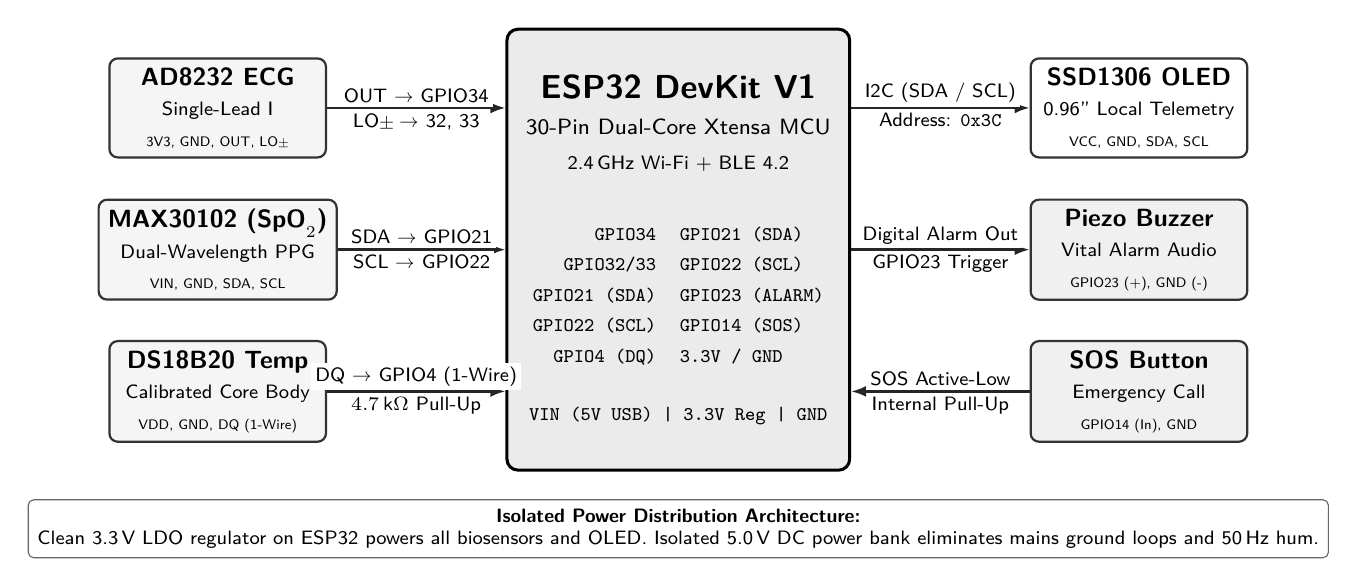
\begin{tikzpicture}[
    font=\sffamily\small,
    mcu/.style={rectangle, rounded corners=4pt, draw=black, fill=black!8, line width=1.1pt, minimum width=4.6cm, minimum height=5.6cm, align=center},
    sensor/.style={rectangle, rounded corners=3pt, draw=black!80, fill=black!4, line width=0.8pt, minimum width=3.4cm, minimum height=1.15cm, align=center},
    disp/.style={rectangle, rounded corners=3pt, draw=black!80, fill=white, line width=0.8pt, minimum width=3.4cm, minimum height=1.15cm, align=center},
    act/.style={rectangle, rounded corners=3pt, draw=black!80, fill=black!6, line width=0.8pt, minimum width=3.4cm, minimum height=1.15cm, align=center},
    wiretag/.style={font=\sffamily\scriptsize, color=black, fill=white, inner sep=1.5pt, align=center},
    sig/.style={line width=0.85pt, -{Latex[length=1.9mm, width=1.4mm]}, draw=black!85}
]

    % Central ESP32 Node
    \node[mcu, minimum width=4.0cm] (esp) at (0, 0) {
        \textbf{\large ESP32 DevKit V1}\\[2pt]
        \footnotesize 30-Pin Dual-Core Xtensa MCU\\[2pt]
        \scriptsize 2.4\,GHz Wi-Fi + BLE 4.2\\[16pt]
        \begin{tabular}{r@{\hspace{0.3cm}}l}
            \scriptsize\texttt{GPIO34} & \scriptsize\texttt{GPIO21 (SDA)} \\
            \scriptsize\texttt{GPIO32/33} & \scriptsize\texttt{GPIO22 (SCL)} \\
            \scriptsize\texttt{GPIO21 (SDA)} & \scriptsize\texttt{GPIO23 (ALARM)} \\
            \scriptsize\texttt{GPIO22 (SCL)} & \scriptsize\texttt{GPIO14 (SOS)} \\
            \scriptsize\texttt{GPIO4 (DQ)} & \scriptsize\texttt{3.3V / GND} \\
        \end{tabular}\\[12pt]
        \texttt{\scriptsize VIN (5V USB) \textbar\ 3.3V Reg \textbar\ GND}
    };

    % Left Peripherals (Sensors) - compact width 2.75cm placed at x = -5.85
    \node[sensor, minimum width=2.75cm] (ad8232) at (-5.85, 1.8) {
        \textbf{AD8232 ECG}\\
        \scriptsize Single-Lead I\\
        \tiny 3V3, GND, OUT, LO$\pm$
    };

    \node[sensor, minimum width=2.75cm] (max30102) at (-5.85, 0.0) {
        \textbf{MAX30102 ($\text{SpO}_2$)}\\
        \scriptsize Dual-Wavelength PPG\\
        \tiny VIN, GND, SDA, SCL
    };

    \node[sensor, minimum width=2.75cm] (ds18b20) at (-5.85, -1.8) {
        \textbf{DS18B20 Temp}\\
        \scriptsize Calibrated Core Body\\
        \tiny VDD, GND, DQ (1-Wire)
    };

    % Right Peripherals (Outputs & Controls) - compact width 2.75cm placed at x = +5.85
    \node[disp, minimum width=2.75cm] (oled) at (5.85, 1.8) {
        \textbf{SSD1306 OLED}\\
        \scriptsize 0.96'' Local Telemetry\\
        \tiny VCC, GND, SDA, SCL
    };

    \node[act, minimum width=2.75cm] (buzzer) at (5.85, 0.0) {
        \textbf{Piezo Buzzer}\\
        \scriptsize Vital Alarm Audio\\
        \tiny GPIO23 (+), GND (-)
    };

    \node[act, minimum width=2.75cm] (button) at (5.85, -1.8) {
        \textbf{SOS Button}\\
        \scriptsize Emergency Call\\
        \tiny GPIO14 (In), GND
    };

    % Left Connections (Sensors -> ESP32)
    \draw[sig] (ad8232.east) -- node[wiretag, above]{OUT $\rightarrow$ GPIO34} node[wiretag, below]{LO$\pm \rightarrow$ 32, 33} (esp.west |- ad8232.east);
    \draw[sig] (max30102.east) -- node[wiretag, above]{SDA $\rightarrow$ GPIO21} node[wiretag, below]{SCL $\rightarrow$ GPIO22} (esp.west |- max30102.east);
    \draw[sig] (ds18b20.east) -- node[wiretag, above]{DQ $\rightarrow$ GPIO4 (1-Wire)} node[wiretag, below]{$4.7\,\text{k}\Omega$ Pull-Up} (esp.west |- ds18b20.east);

    % Right Connections (ESP32 -> Outputs)
    \draw[sig] (esp.east |- oled.west) -- node[wiretag, above]{I2C (SDA / SCL)} node[wiretag, below]{Address: \texttt{0x3C}} (oled.west);
    \draw[sig] (esp.east |- buzzer.west) -- node[wiretag, above]{Digital Alarm Out} node[wiretag, below]{GPIO23 Trigger} (buzzer.west);
    \draw[sig] (button.west) -- node[wiretag, above]{SOS Active-Low} node[wiretag, below]{Internal Pull-Up} (esp.east |- button.west);

    % Bottom Power Rails Box
    \node[rectangle, draw=black!60, fill=white, rounded corners=2pt, font=\scriptsize\sffamily, align=center, below=0.35cm of esp] (pwr) {
        \textbf{Isolated Power Distribution Architecture:}\\
        \scriptsize Clean 3.3\,V LDO regulator on ESP32 powers all biosensors and OLED. Isolated 5.0\,V DC power bank eliminates mains ground loops and 50\,Hz hum.
    };

\end{tikzpicture}%
}
\end{tcolorbox}
\vspace{-0.2cm}
\caption{Complete Hardware Circuit Interconnection and ESP32 Pin Allocation Schematic.}
\label{fig:circuit_schematic}
\end{figure}

Table~\ref{tab:pin_map} summarizes the verified hardware GPIO pin allocation on the ESP32.

\vspace{0.08cm}
\begin{table}[htbp]
\centering
\footnotesize
\setlength{\tabcolsep}{4.5pt}
\renewcommand{\arraystretch}{1.08}
\setlength{\tblavail}{\dimexpr\linewidth - 8\tabcolsep - 5\arrayrulewidth\relax}
\setlength{\wA}{0.20\tblavail}
\setlength{\wB}{0.22\tblavail}
\setlength{\wC}{0.28\tblavail}
\setlength{\wD}{0.30\tblavail}
\begin{tabular}{|B{\wA}|L{\wB}|L{\wC}|L{\wD}|}
    \hline
    \multicolumn{1}{|M{\wA}|}{\textbf{ESP32 Pin}} & \multicolumn{1}{M{\wB}|}{\textbf{Connected Peripheral}} & \multicolumn{1}{M{\wC}|}{\textbf{Signal Function}} & \multicolumn{1}{M{\wD}|}{\textbf{Hardware Notes}} \\
    \hline
    GPIO 34 & AD8232 OUTPUT & Analog ECG input (ADC1\_CH6) & Input-only pin; low noise channel \\
    \hline
    GPIO 32, 33 & AD8232 LO+, LO- & Leads-Off detection & Digital inputs; flags detached leads \\
    \hline
    GPIO 21 & MAX30102 / OLED & I2C Serial Data (SDA) & Shared I2C bus (\texttt{0x57} \& \texttt{0x3C}) \\
    \hline
    GPIO 22 & MAX30102 / OLED & I2C Serial Clock (SCL) & 400\,kHz standard I2C clock \\
    \hline
    GPIO 4 & DS18B20 DQ & 1-Wire bidirectional data & Requires external $4.7\,\text{k}\Omega$ pull-up to 3.3\,V \\
    \hline
    GPIO 23 & Active Piezo Buzzer & Audible alarm trigger & High = Alarm Active, Low = Silent \\
    \hline
    GPIO 14 & SOS Push Button & Emergency alert trigger & Active-low input with internal pull-up \\
    \hline
\end{tabular}
\caption{ESP32 GPIO Pin Assignment and Peripheral Mapping.}
\label{tab:pin_map}
\end{table}
\clearpage

% ==============================================================================
% PAGE 7: SECTION 3 — END-TO-END SYSTEM WORKFLOW AND ARCHITECTURE
% ==============================================================================
\section{End-to-End System Workflow and Architecture}
\label{sec:system_workflow}

\subsection{Architectural Layer Overview}
The SmartHealth IoT system is structured into five cohesive architectural layers:
\begin{enumerate}
    \item \textbf{Perception / Edge Sensing Layer:} Biosensors (AD8232, MAX30102, DS18B20) attached to the patient acquire analog and optical physiological signals.
    \item \textbf{Edge Computing Layer:} The ESP32 digitizes ECG signals, performs optical pulse calculations, formats batched JSON packets, manages local fallback alarms, and transmits data over Wi-Fi.
    \item \textbf{Backend Ingestion Layer:} A Python FastAPI server validates incoming packets via Pydantic, controls device authentication, coordinates persistence, and manages active client connections.
    \item \textbf{Data \& Analytical Layer:} MongoDB Atlas provides persistent time-series storage, while in-memory scikit-learn models perform multivariate anomaly detection and vital trend prediction.
    \item \textbf{Presentation Layer:} A responsive React single-page dashboard renders live vital cards and animates an oscilloscope-style ECG trace in real time via WebSockets.
\end{enumerate}

\subsection{End-to-End Telemetry Data Sequence}
Figure~\ref{fig:e2e_sequence} charts the lifecycle of physiological data from sensor acquisition to browser display in monochrome format.

\vspace{0.15cm}
\begin{figure}[htbp]
\centering
\begin{tcolorbox}[tikzbox, title={End-to-End Telemetry Data Flow Sequence Diagram}, width=\linewidth]
\centering
\resizebox{\linewidth}{!}{%
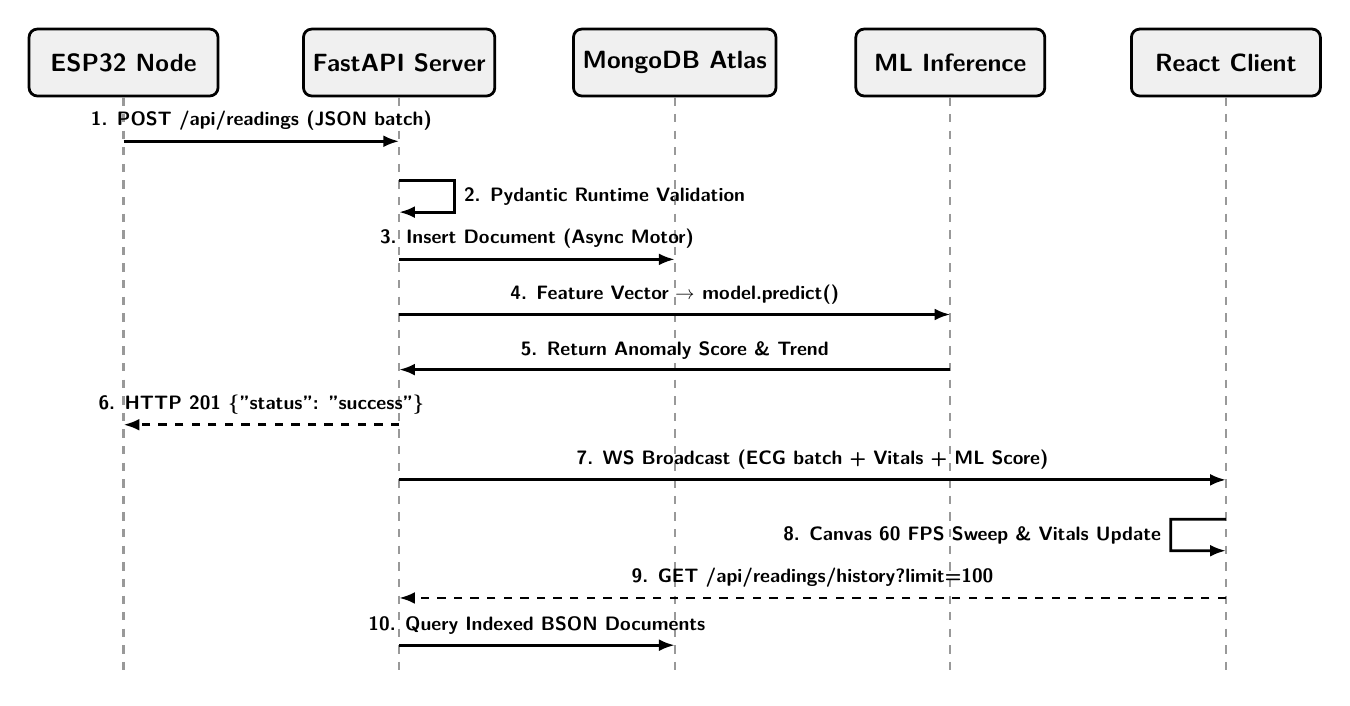
\begin{tikzpicture}[
    font=\sffamily\small,
    box/.style={rectangle, rounded corners=3pt, draw=black, fill=black!6, line width=1pt, align=center, minimum width=2.4cm, minimum height=0.85cm},
    line/.style={draw=black!40, dashed, line width=0.8pt},
    msg/.style={-{Latex[length=2.0mm, width=1.5mm]}, line width=1.0pt, color=black}
]

    % Entity Headers
    \node[box] (p_esp) at (0,0) {\textbf{ESP32 Node}};
    \node[box] (p_api) at (3.5,0) {\textbf{FastAPI Server}};
    \node[box] (p_db) at (7.0,0) {\textbf{MongoDB Atlas}};
    \node[box] (p_ml) at (10.5,0) {\textbf{ML Inference}};
    \node[box] (p_react) at (14.0,0) {\textbf{React Client}};

    % Lifelines
    \draw[line] (p_esp) -- ++(0,-7.8);
    \draw[line] (p_api) -- ++(0,-7.8);
    \draw[line] (p_db) -- ++(0,-7.8);
    \draw[line] (p_ml) -- ++(0,-7.8);
    \draw[line] (p_react) -- ++(0,-7.8);

    % Steps
    \draw[msg] (0,-1.0) -- node[above, font=\scriptsize\sffamily]{\textbf{1. POST /api/readings (JSON batch)}} (3.5,-1.0);
    
    % Step 2: Self-loop on FastAPI
    \draw[msg] (3.5,-1.5) -- ++(0.7,0) -- ++(0,-0.4) -- (3.5,-1.9);
    \node[right, font=\scriptsize\sffamily] at (4.2,-1.7) {\textbf{2. Pydantic Runtime Validation}};
    
    % Storage & ML
    \draw[msg] (3.5,-2.5) -- node[above, font=\scriptsize\sffamily]{\textbf{3. Insert Document (Async Motor)}} (7.0,-2.5);
    \draw[msg] (3.5,-3.2) -- node[above, font=\scriptsize\sffamily]{\textbf{4. Feature Vector $\rightarrow$ model.predict()}} (10.5,-3.2);
    \draw[msg] (10.5,-3.9) -- node[above, font=\scriptsize\sffamily]{\textbf{5. Return Anomaly Score \& Trend}} (3.5,-3.9);

    % Response to ESP32
    \draw[msg, dashed] (3.5,-4.6) -- node[above, font=\scriptsize\sffamily]{\textbf{6. HTTP 201 \{"status": "success"\}}} (0,-4.6);

    % WebSocket Broadcast
    \draw[msg] (3.5,-5.3) -- node[above, font=\scriptsize\sffamily]{\textbf{7. WS Broadcast (ECG batch + Vitals + ML Score)}} (14.0,-5.3);
    
    % Step 8: Self-loop on React Client
    \draw[msg] (14.0,-5.8) -- ++(-0.7,0) -- ++(0,-0.4) -- (14.0,-6.2);
    \node[left, font=\scriptsize\sffamily] at (13.3,-6.0) {\textbf{8. Canvas 60 FPS Sweep \& Vitals Update}};

    % History Query
    \draw[msg, dashed] (14.0,-6.8) -- node[above, font=\scriptsize\sffamily]{\textbf{9. GET /api/readings/history?limit=100}} (3.5,-6.8);
    \draw[msg] (3.5,-7.4) -- node[above, font=\scriptsize\sffamily]{\textbf{10. Query Indexed BSON Documents}} (7.0,-7.4);

\end{tikzpicture}%
}
\end{tcolorbox}
\vspace{-0.2cm}
\caption{End-to-End Sequence Diagram of Multi-Parameter Telemetry Flow.}
\label{fig:e2e_sequence}
\end{figure}
\clearpage

% ==============================================================================
% PAGE 8: SECTION 4 — EMBEDDED FIRMWARE WORKFLOW AND BATCHING PROTOCOL
% ==============================================================================
\section{Embedded Firmware Workflow and Batching Protocol}
\label{sec:firmware_workflow}

\subsection{Multi-Rate Cyclic Executive and Sampling Architecture}
The ESP32 firmware executes a non-blocking cyclic executive loop. The system satisfies two conflicting timing demands: (i) sampling high-frequency analog ECG waveforms at 100\,Hz with minimal jitter, and (ii) dispatching HTTP network requests over Wi-Fi without blocking execution.

\textbf{The Chunked Batching Protocol:} At 100\,Hz, sending one HTTP request per ECG point would generate 100 TCP handshakes and HTTP header frames per second, causing buffer overruns. Instead, the firmware accumulates 50 consecutive ADC samples in an internal ring buffer over 250\,ms. When full, this array is bundled with the latest $\text{SpO}_2$, heart rate, and temperature readings into a single JSON payload. This reduces network transmissions to 4 requests per second while preserving 100\,Hz waveform fidelity.

\vspace{0.08cm}
\begin{figure}[H]
\centering
\begin{tcolorbox}[tikzbox, title={ESP32 Embedded Firmware Execution and Telemetry Batching Flowchart}, left=4pt, right=4pt, top=3pt, bottom=3pt, width=\linewidth]
\centering
\resizebox{0.86\linewidth}{!}{%
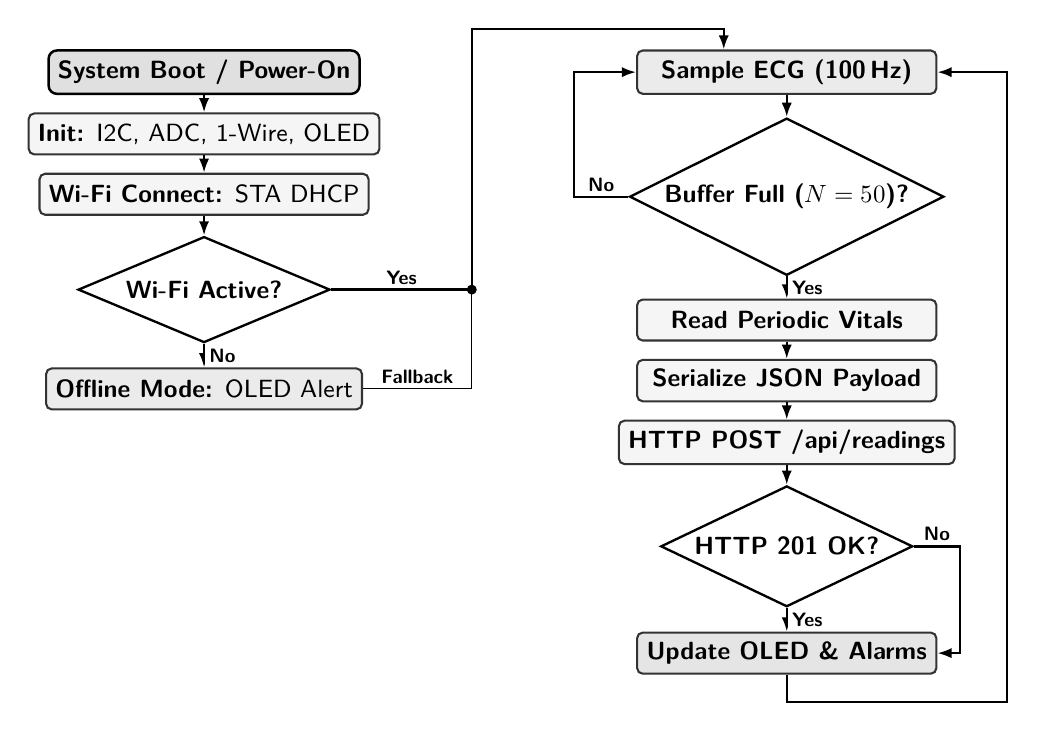
\begin{tikzpicture}[
    font=\sffamily\small,
    startstop/.style={rectangle, rounded corners=3pt, draw=black, fill=black!12, line width=0.9pt, minimum width=3.8cm, minimum height=0.52cm, align=center},
    process/.style={rectangle, rounded corners=2pt, draw=black!80, fill=black!4, line width=0.75pt, minimum width=3.8cm, minimum height=0.52cm, align=center},
    decision/.style={diamond, aspect=2.0, draw=black, fill=white, line width=0.85pt, align=center, inner sep=1.2pt, minimum width=3.2cm},
    arr/.style={-{Latex[length=1.8mm, width=1.3mm]}, line width=0.85pt, color=black},
    lbl/.style={font=\scriptsize\bfseries\sffamily, fill=white, inner sep=1.5pt}
]

    % Stage I: System Initialization & Wi-Fi Setup (Left Column, x = -3.8)
    \node[startstop] (start) at (-3.8, 2.7) {\textbf{System Boot / Power-On}};
    \node[process, below=0.22cm of start] (init) {\textbf{Init: }I2C, ADC, 1-Wire, OLED};
    \node[process, below=0.22cm of init] (wifi) {\textbf{Wi-Fi Connect: }STA DHCP};
    \node[decision, below=0.25cm of wifi] (wcheck) {\textbf{Wi-Fi Active?}};
    \node[process, fill=black!8, below=0.30cm of wcheck] (offline) {\textbf{Offline Mode: }OLED Alert};

    % Stage II: Cyclic Sampling & Batch Telemetry Loop (Right Column, x = 3.6)
    \node[process, fill=black!8] (sample) at (3.6, 2.7) {\textbf{Sample ECG (100\,Hz)}};
    \node[decision, below=0.28cm of sample] (bcheck) {\textbf{Buffer Full ($N = 50$)?}};
    \node[process, below=0.28cm of bcheck] (vitals) {\textbf{Read Periodic Vitals}};
    \node[process, below=0.22cm of vitals] (batch) {\textbf{Serialize JSON Payload}};
    \node[process, below=0.22cm of batch] (post) {\textbf{HTTP POST /api/readings}};
    \node[decision, below=0.25cm of post] (hcheck) {\textbf{HTTP 201 OK?}};
    \node[process, fill=black!10, below=0.30cm of hcheck] (alert) {\textbf{Update OLED \& Alarms}};

    % Connections: Stage I Downward Flow
    \draw[arr] (start) -- (init);
    \draw[arr] (init) -- (wifi);
    \draw[arr] (wifi) -- (wcheck);
    \draw[arr] (wcheck) -- node[lbl, right]{No} (offline);
    
    % Transition from Stage I to Stage II (Startup Entry via North: x = -0.4 to y = 3.25)
    \draw[arr] (wcheck.east) -- node[lbl, above]{Yes} (-0.4, 0 |- wcheck.east) -- (-0.4, 3.25) -- ([xshift=-0.8cm]sample.north |- 0, 3.25) -- ([xshift=-0.8cm]sample.north);
    \draw (offline.east) -- node[lbl, above]{Fallback} (-0.4, 0 |- offline.east) -- (-0.4, 0 |- wcheck.east);
    \fill[black] (-0.4, 0 |- wcheck.east) circle (1.8pt);

    % Connections: Stage II Internal 100Hz Loop (Dedicated Return via West at x = 0.9)
    \draw[arr] (sample) -- (bcheck);
    \draw[arr] (bcheck) -- node[lbl, right]{Yes} (vitals);
    \draw[arr] (bcheck.west) -- node[lbl, above]{No} (0.9, 0 |- bcheck.west) |- (sample.west);

    % Stage II Dispatch Chain Downward Flow
    \draw[arr] (vitals) -- (batch);
    \draw[arr] (batch) -- (post);
    \draw[arr] (post) -- (hcheck);
    \draw[arr] (hcheck) -- node[lbl, right]{Yes} (alert);
    
    % HTTP Failure (No) Bypass to Update OLED & Alarms via x = 5.8
    \draw[arr] (hcheck.east) -- node[lbl, above]{No} (5.8, 0 |- hcheck.east) |- (alert.east);

    % Global Loop Return along Outer Right Perimeter (x = 6.4)
    \draw[arr] (alert.south) -- ++(0, -0.35) -| (6.4, 0) |- (sample.east);

\end{tikzpicture}%
}
\end{tcolorbox}
\vspace{-0.25cm}
\caption{ESP32 Embedded Firmware Execution and Telemetry Batching Flowchart.}
\label{fig:firmware_flowchart}
\end{figure}

\subsection{Canonical JSON Telemetry Payload Structure}
The ESP32 formats sensor readings into the canonical JSON schema below:
\begin{tcolorbox}[colback=black!3, colframe=black!60, arc=2pt, boxrule=0.6pt, left=5pt, right=5pt, top=2pt, bottom=2pt]
\footnotesize\ttfamily
\{\\
\quad "device\_id": "ESP32\_001", "heart\_rate": 76.0, "spo2": 98.0, "temperature": 36.7,\\
\quad "ecg\_samples": [512, 518, 525, 540, 610, 720, 850, 650, 530, 515, ...]\\
\}
\end{tcolorbox}
\clearpage

% ==============================================================================
% PAGE 9: SECTION 5 — BACKEND INGESTION, API AND DATABASE WORKFLOW
% ==============================================================================
\section{Backend Ingestion, API and Database Workflow}
\label{sec:backend_workflow}

\subsection{FastAPI Ingestion Architecture and Processing Pipeline}
The backend runs on \textbf{Python FastAPI} using the ASGI server Uvicorn. When a payload arrives at \texttt{POST /api/readings}, FastAPI executes an asynchronous eight-stage pipeline, illustrated in Figure~\ref{fig:backend_pipeline}.

\vspace{0.12cm}
\begin{figure}[H]
\centering
\begin{tcolorbox}[tikzbox, title={FastAPI Telemetry Ingestion and Real-Time Processing Pipeline}, width=\linewidth]
\centering
\resizebox{\linewidth}{!}{%
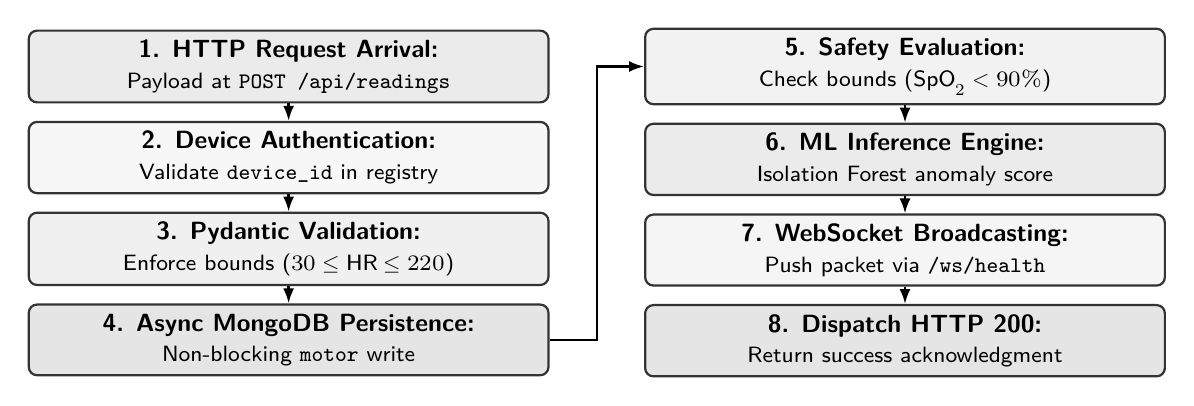
\begin{tikzpicture}[
    font=\sffamily\small,
    stepnode/.style={rectangle, rounded corners=3pt, draw=black!80, fill=black!4, line width=0.8pt, minimum width=6.6cm, minimum height=0.70cm, align=center},
    arr/.style={-{Latex[length=1.9mm, width=1.4mm]}, line width=0.85pt, color=black}
]

    % Left Column (Steps 1 to 4)
    \node[stepnode, fill=black!8] (s1) at (0,0) {\textbf{1. HTTP Request Arrival:}\\\footnotesize Payload at \texttt{POST /api/readings}};
    \node[stepnode, fill=black!3, below=0.22cm of s1] (s2) {\textbf{2. Device Authentication:}\\\footnotesize Validate \texttt{device\_id} in registry};
    \node[stepnode, fill=black!6, below=0.22cm of s2] (s3) {\textbf{3. Pydantic Validation:}\\\footnotesize Enforce bounds ($30 \le \text{HR} \le 220$)};
    \node[stepnode, fill=black!10, below=0.22cm of s3] (s4) {\textbf{4. Async MongoDB Persistence:}\\\footnotesize Non-blocking \texttt{motor} write};

    % Right Column (Steps 5 to 8)
    \node[stepnode, fill=black!5, right=1.2cm of s1] (s5) {\textbf{5. Safety Evaluation:}\\\footnotesize Check bounds ($\text{SpO}_2 < 90\%$)};
    \node[stepnode, fill=black!8, below=0.22cm of s5] (s6) {\textbf{6. ML Inference Engine:}\\\footnotesize Isolation Forest anomaly score};
    \node[stepnode, fill=black!4, below=0.22cm of s6] (s7) {\textbf{7. WebSocket Broadcasting:}\\\footnotesize Push packet via \texttt{/ws/health}};
    \node[stepnode, fill=black!10, below=0.22cm of s7] (s8) {\textbf{8. Dispatch HTTP 200:}\\\footnotesize Return success acknowledgment};

    % Left connections
    \draw[arr] (s1) -- (s2);
    \draw[arr] (s2) -- (s3);
    \draw[arr] (s3) -- (s4);

    % Bridge from step 4 to 5
    \draw[arr] (s4.east) -- ++(0.6,0) |- (s5.west);

    % Right connections
    \draw[arr] (s5) -- (s6);
    \draw[arr] (s6) -- (s7);
    \draw[arr] (s7) -- (s8);

\end{tikzpicture}%
}
\end{tcolorbox}
\vspace{-0.2cm}
\caption{FastAPI Ingestion and Real-Time Analytics Pipeline.}
\label{fig:backend_pipeline}
\end{figure}

\subsection{REST API and WebSocket Interface Specifications}
Table~\ref{tab:api_specs} defines the endpoints exposed by the FastAPI server.

\vspace{0.08cm}
\begin{table}[H]
\centering
\small
\setlength{\tabcolsep}{4.5pt}
\renewcommand{\arraystretch}{1.12}
\setlength{\tblavail}{\dimexpr\linewidth - 8\tabcolsep - 5\arrayrulewidth\relax}
\setlength{\wA}{0.12\tblavail}
\setlength{\wB}{0.34\tblavail}
\setlength{\wC}{0.20\tblavail}
\setlength{\wD}{0.34\tblavail}
\begin{tabular}{|B{\wA}|L{\wB}|L{\wC}|L{\wD}|}
    \hline
    \multicolumn{1}{|M{\wA}|}{\textbf{Verb}} &
    \multicolumn{1}{M{\wB}|}{\textbf{Route Path}} &
    \multicolumn{1}{M{\wC}|}{\textbf{Input Parameters}} &
    \multicolumn{1}{M{\wD}|}{\textbf{Output Description \& Status}} \\
    \hline
    \texttt{POST} & \texttt{/api/readings} & JSON Body (\texttt{HealthReading}) & Returns \texttt{\{"status": "success"\}} (201 Created) \\
    \hline
    \texttt{GET} & \texttt{/api/readings/latest} & Query: \texttt{?device\_id=...} & Returns latest vitals, anomaly score, status (200 OK) \\
    \hline
    \texttt{GET} & \texttt{/api/readings/history} & Query: \texttt{?limit=100} & Paginated historical readings array (200 OK) \\
    \hline
    \texttt{POST} & \texttt{/api/devices/register} & JSON Body (\texttt{device\_id}) & Registers hardware node; returns key (200 OK) \\
    \hline
    \texttt{GET} & \texttt{/api/predictions/latest} & Query: \texttt{?device\_id=...} & Returns current ML anomaly score \& trend (200 OK) \\
    \hline
    \texttt{WS} & \texttt{/ws/health} & WebSocket handshake & Full-duplex JSON stream of ECG \& vitals (101 Switching) \\
    \hline
\end{tabular}
\caption{REST API and WebSocket Endpoint Specifications.}
\label{tab:api_specs}
\end{table}
\clearpage

% ==============================================================================
% PAGE 10: SECTION 5 (CONT.) — DATABASE SCHEMA & DATA MODELS
% ==============================================================================
\subsection{MongoDB Document Schema Design}
The database layer uses \textbf{MongoDB Atlas} via the asynchronous Python driver \texttt{motor}. The document-oriented BSON format naturally accommodates variable-length ECG sample arrays alongside scalar vitals. Table~\ref{tab:mongo_schema} details the four collections.

\vspace{0.08cm}
\begin{table}[htbp]
\centering
\footnotesize
\setlength{\tabcolsep}{4.5pt}
\renewcommand{\arraystretch}{1.04}
\setlength{\tblavail}{\dimexpr\linewidth - 8\tabcolsep - 5\arrayrulewidth\relax}
\setlength{\wA}{0.18\tblavail}
\setlength{\wB}{0.22\tblavail}
\setlength{\wC}{0.18\tblavail}
\setlength{\wD}{0.42\tblavail}
\begin{tabular}{|B{\wA}|L{\wB}|L{\wC}|L{\wD}|}
    \hline
    \multicolumn{1}{|M{\wA}|}{\textbf{Collection}} &
    \multicolumn{1}{M{\wB}|}{\textbf{Field Name}} &
    \multicolumn{1}{M{\wC}|}{\textbf{BSON Type}} &
    \multicolumn{1}{M{\wD}|}{\textbf{Field Description and Indexing Rules}} \\
    \hline
    \textbf{readings} & \texttt{\_id} & \texttt{ObjectId} & Unique MongoDB document identifier (Primary Key) \\
    & \texttt{device\_id} & \texttt{String} & Node identifier (e.g., \texttt{"ESP32\_001"}); indexed \\
    & \texttt{heart\_rate} & \texttt{Double} & Heart rate in BPM ($30.0 - 220.0$) \\
    & \texttt{spo2} & \texttt{Double} & Blood oxygen saturation percentage ($70.0 - 100.0$) \\
    & \texttt{temperature} & \texttt{Double} & Body surface temperature in Celsius ($30.0 - 45.0$) \\
    & \texttt{ecg\_samples} & \texttt{Array[Int32]} & Batch of digitized AD8232 ADC samples (50 ints) \\
    & \texttt{timestamp} & \texttt{Date} & UTC ISO-8601 insertion time; compound index \\
    \hline
    \textbf{devices} & \texttt{device\_id} & \texttt{String} & Unique hardware node serial identifier (Indexed) \\
    & \texttt{firmware\_rev} & \texttt{String} & Installed firmware version (e.g., \texttt{"v1.0.4"}) \\
    & \texttt{status} & \texttt{String} & Node state: \texttt{"ONLINE"}, \texttt{"OFFLINE"}, \texttt{"ERROR"} \\
    & \texttt{last\_seen} & \texttt{Date} & Timestamp of most recent valid packet transmission \\
    \hline
    \textbf{alerts} & \texttt{alert\_id} & \texttt{ObjectId} & Unique alarm incident identifier \\
    & \texttt{device\_id} & \texttt{String} & Originating hardware unit identifier \\
    & \texttt{severity} & \texttt{String} & Incident severity level: \texttt{"WARNING"}, \texttt{"CRITICAL"} \\
    & \texttt{message} & \texttt{String} & Alarm description (e.g., \texttt{"Low SpO2: 88\% detected"}) \\
    & \texttt{timestamp} & \texttt{Date} & Timestamp when alert was logged \\
    \hline
    \textbf{predictions} & \texttt{pred\_id} & \texttt{ObjectId} & Unique analytical record identifier \\
    & \texttt{anomaly\_score} & \texttt{Double} & Normalized Isolation Forest score ($0.0 - 1.0$) \\
    & \texttt{trend\_vector} & \texttt{Object} & Vital slopes: \texttt{\{"hr\_slope", "spo2\_slope"\}} \\
    & \texttt{timestamp} & \texttt{Date} & Timestamp corresponding to evaluated inference window \\
    \hline
\end{tabular}
\caption{MongoDB Document Collections and Field Definitions.}
\label{tab:mongo_schema}
\end{table}

\subsection{Pydantic Data Models and Schema Validation}
FastAPI automatically enforces data integrity through Pydantic models. Incoming payloads with out-of-range numerical values or corrupt data types are rejected at the network boundary with HTTP 422, shielding the database and ML pipeline.

\begin{tcolorbox}[colback=black!3, colframe=black!60, arc=2pt, boxrule=0.6pt, left=5pt, right=5pt, top=2pt, bottom=2pt]
\footnotesize\ttfamily
class HealthReading(BaseModel):\\
\quad device\_id: str = Field(..., example="ESP32\_001")\\
\quad heart\_rate: float = Field(..., ge=30.0, le=220.0)\\
\quad spo2: float = Field(..., ge=70.0, le=100.0)\\
\quad temperature: float = Field(..., ge=30.0, le=45.0)\\
\quad ecg\_samples: List[int] = Field(..., min\_items=10, max\_items=200)
\end{tcolorbox}
\clearpage

% ==============================================================================
% PAGE 11: SECTION 6 — MACHINE LEARNING WORKFLOW: ANOMALY AND TRENDS
% ==============================================================================
\section{Machine Learning Workflow: Anomaly and Trends}
\label{sec:ml_workflow}

\subsection{Decoupled Machine Learning Architecture}
To ensure system stability, \textbf{offline model training} is kept completely separate from \textbf{real-time cloud inference}, as shown in Figure~\ref{fig:ml_workflow}.
\begin{itemize}
    \item \textbf{Offline Training (\texttt{ml/train.py}):} The model is trained offline on baseline physiological datasets using scikit-learn. The trained model is serialized into \texttt{model.pkl} via Joblib.
    \item \textbf{Online Inference (\texttt{prediction\_service.py}):} During FastAPI startup, \texttt{model.pkl} is loaded into RAM once. Incoming sensor readings are transformed into feature vectors and scored in sub-5\,ms, with results returned during the active request cycle.
\end{itemize}

\vspace{0.15cm}
\begin{figure}[htbp]
\centering
\begin{tcolorbox}[tikzbox, title={Decoupled Machine Learning Architecture: Offline Training vs. Online Inference}, width=\linewidth]
\centering
\resizebox{\linewidth}{!}{%
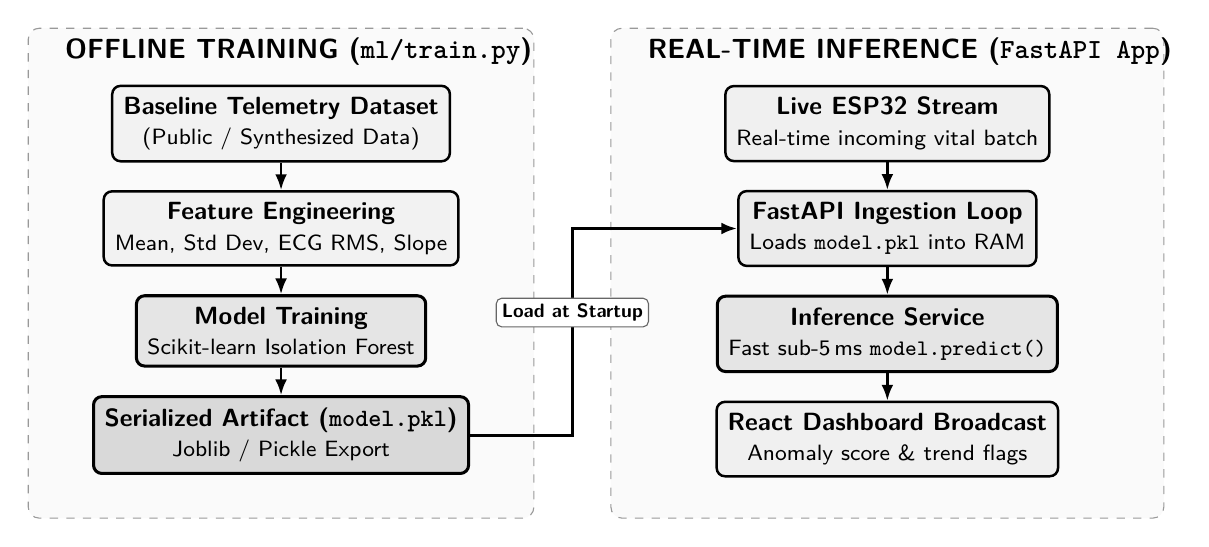
\begin{tikzpicture}[
    font=\sffamily\small,
    box/.style={rectangle, rounded corners=3pt, draw=black, fill=black!5, line width=0.9pt, align=center, minimum height=0.85cm, inner sep=4pt},
    mlbox/.style={box, draw=black, fill=black!10, line width=1.1pt},
    arr/.style={-{Latex[length=2.0mm, width=1.5mm]}, line width=0.9pt, color=black}
]

    % Training Pipeline Subgraph (Left)
    \node[draw=black!40, dashed, fill=black!2, rounded corners=4pt, inner sep=6pt, fit={(0.2,0.2) (6.2,-5.6)}] (trainbg) {};
    \node[font=\bfseries\sffamily\color{black}, anchor=north west] at (trainbg.north west) {\quad OFFLINE TRAINING (\texttt{ml/train.py})};

    \node[box] (dset) at (3.2,-0.8) {\textbf{Baseline Telemetry Dataset}\\\footnotesize (Public / Synthesized Data)};
    \node[box, below=0.35cm of dset] (feat) {\textbf{Feature Engineering}\\\footnotesize Mean, Std Dev, ECG RMS, Slope};
    \node[mlbox, below=0.35cm of feat] (train) {\textbf{Model Training}\\\footnotesize Scikit-learn Isolation Forest};
    \node[mlbox, fill=black!15, below=0.35cm of train] (pkl) {\textbf{Serialized Artifact (\texttt{model.pkl})}\\\footnotesize Joblib / Pickle Export};

    % Inference Pipeline Subgraph (Right)
    \node[draw=black!40, dashed, fill=black!2, rounded corners=4pt, inner sep=6pt, fit={(7.6,0.2) (14.2,-5.6)}] (infbg) {};
    \node[font=\bfseries\sffamily\color{black}, anchor=north west] at (infbg.north west) {\quad REAL-TIME INFERENCE (\texttt{FastAPI App})};

    \node[box, fill=black!6] (esp) at (10.9,-0.8) {\textbf{Live ESP32 Stream}\\\footnotesize Real-time incoming vital batch};
    \node[box, fill=black!8, below=0.35cm of esp] (fastapi) {\textbf{FastAPI Ingestion Loop}\\\footnotesize Loads \texttt{model.pkl} into RAM};
    \node[mlbox, below=0.35cm of fastapi] (infer) {\textbf{Inference Service}\\\footnotesize Fast sub-5\,ms \texttt{model.predict()}};
    \node[box, fill=black!6, below=0.35cm of infer] (dash) {\textbf{React Dashboard Broadcast}\\\footnotesize Anomaly score \& trend flags};

    % Training Connections
    \draw[arr] (dset) -- (feat);
    \draw[arr] (feat) -- (train);
    \draw[arr] (train) -- (pkl);

    % Bridge Between Training and Inference (Centered Aisle at x = 6.9)
    \draw[arr, line width=1.1pt] (pkl.east) -- (6.9, 0 |- pkl.east) -- (6.9, 0 |- fastapi.west) -- (fastapi.west);
    \node[font=\scriptsize\bfseries\sffamily, fill=white, inner sep=2pt, draw=black!60, rounded corners=2pt] at (6.9, -3.2) {Load at Startup};

    % Inference Connections
    \draw[arr] (esp) -- (fastapi);
    \draw[arr] (fastapi) -- (infer);
    \draw[arr] (infer) -- (dash);

\end{tikzpicture}%
}
\end{tcolorbox}
\vspace{-0.2cm}
\caption{Decoupled Machine Learning Workflow: Offline Training vs. Online Inference.}
\label{fig:ml_workflow}
\end{figure}

\subsection{Multivariate Anomaly Detection and Trend Projection}
\textbf{Feature 1: Isolation Forest Anomaly Detection:} Traditional threshold checks only flag values after they cross fixed limits. The Isolation Forest isolates anomalies using random recursive partitioning. Feature vectors are extracted across a sliding 30-second window:
\begin{equation}
    \mathbf{x} = \left[ \mu_{\text{HR}}, \; \sigma_{\text{HR}}, \; \mu_{\text{SpO}_2}, \; \mu_{\text{Temp}}, \; \Delta \text{Temp}, \; \text{RMS}_{\text{ECG}} \right]
\end{equation}
The model computes a normalized anomaly score from $0.0$ (nominal) to $1.0$ (high anomaly).

\textbf{Feature 2: Multi-Vital Trend Projection:} The system calculates linear slopes ($\frac{d\text{HR}}{dt}$, $\frac{d\text{SpO}_2}{dt}$, $\frac{d\text{Temp}}{dt}$) over sliding 15-minute buffers. For instance, a rising heart rate combined with declining oxygenation triggers an elevated risk indicator before any single variable hits a critical threshold.
\clearpage

% ==============================================================================
% PAGE 12: SECTION 7 — FRONTEND REAL-TIME MONITORING DASHBOARD WORKFLOW
% ==============================================================================
\section{Frontend Real-Time Monitoring Dashboard Workflow}
\label{sec:frontend_workflow}

\subsection{React Dashboard Architecture and State Management}
The user interface is built as a single-page application using \textbf{React 19}, \textbf{Vite 8}, and clean CSS adhering to the \textbf{impeccable.style} design standard. It communicates via two channels:
\begin{enumerate}
    \item \textbf{Full-Duplex WebSocket Client (\texttt{/ws/health}):} Continuously receives live 50-sample ECG arrays, updated vitals, and ML anomaly indices without polling latency.
    \item \textbf{Asynchronous REST Client (Axios):} Fetches historical telemetry records and patient metadata on demand.
\end{enumerate}

\subsection{Component Hierarchy and State Distribution Tree}
Figure~\ref{fig:component_tree} shows the React component hierarchy in monochrome format.

\vspace{0.15cm}
\begin{figure}[htbp]
\centering
\begin{tcolorbox}[tikzbox, title={React Component Hierarchy and State Flow Tree}, width=\linewidth]
\centering
\resizebox{\linewidth}{!}{%
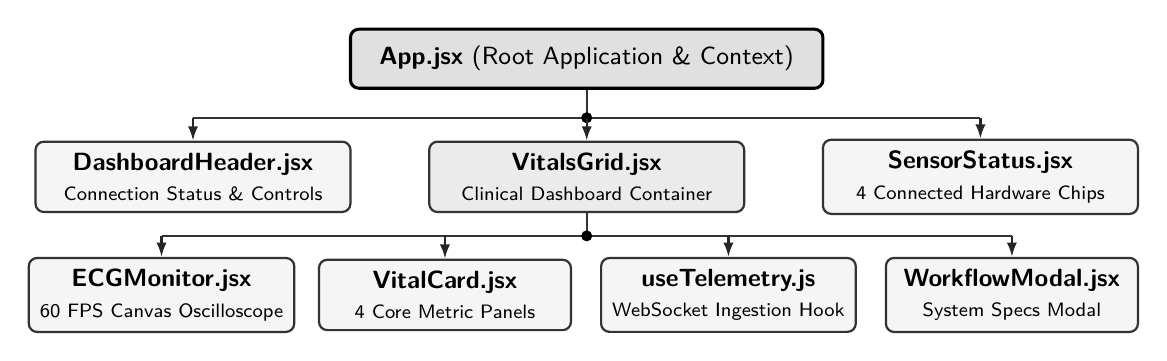
\begin{tikzpicture}[
    font=\sffamily\small,
    cnode/.style={rectangle, rounded corners=3pt, draw=black!80, fill=black!4, line width=0.8pt, align=center, minimum height=0.75cm, inner sep=4pt},
    edge/.style={draw=black!80, line width=0.85pt},
    drop/.style={-{Latex[length=1.8mm, width=1.3mm]}, draw=black!85, line width=0.85pt}
]

    % Tree Nodes
    \node[cnode, fill=black!12, draw=black, line width=1.1pt, minimum width=6.0cm] (app) at (0, 3.0) {\textbf{App.jsx} (Root Application \& Context)};
    
    % Level 2 (Horizontal span: -5.0, 0, +5.0)
    \node[cnode, minimum width=4.0cm] (nav) at (-5.0, 1.5) {\textbf{DashboardHeader.jsx}\\\scriptsize Connection Status \& Controls};
    \node[cnode, fill=black!8, minimum width=4.0cm] (dash) at (0, 1.5) {\textbf{VitalsGrid.jsx}\\\scriptsize Clinical Dashboard Container};
    \node[cnode, minimum width=4.0cm] (hist) at (5.0, 1.5) {\textbf{SensorStatus.jsx}\\\scriptsize 4 Connected Hardware Chips};

    % Level 3 Leaves under VitalsGrid (Span: -5.4, -1.8, +1.8, +5.4)
    \node[cnode, minimum width=3.2cm] (ecg) at (-5.4, 0.0) {\textbf{ECGMonitor.jsx}\\\scriptsize 60 FPS Canvas Oscilloscope};
    \node[cnode, minimum width=3.2cm] (cards) at (-1.8, 0.0) {\textbf{VitalCard.jsx}\\\scriptsize 4 Core Metric Panels};
    \node[cnode, minimum width=3.2cm] (pred) at (1.8, 0.0) {\textbf{useTelemetry.js}\\\scriptsize WebSocket Ingestion Hook};
    \node[cnode, minimum width=3.2cm] (alert) at (5.4, 0.0) {\textbf{WorkflowModal.jsx}\\\scriptsize System Specs Modal};

    % Orthogonal Bus Level 1
    \draw[edge] (app.south) -- (0, 2.25);
    \draw[edge] (-5.0, 2.25) -- (5.0, 2.25);
    \fill[black] (0, 2.25) circle (2.0pt);
    \draw[drop] (-5.0, 2.25) -- (nav.north);
    \draw[drop] (0, 2.25) -- (dash.north);
    \draw[drop] (5.0, 2.25) -- (hist.north);

    % Orthogonal Bus Level 2
    \draw[edge] (dash.south) -- (0, 0.75);
    \draw[edge] (-5.4, 0.75) -- (5.4, 0.75);
    \fill[black] (0, 0.75) circle (2.0pt);
    \draw[drop] (-5.4, 0.75) -- (ecg.north);
    \draw[drop] (-1.8, 0.75) -- (cards.north);
    \draw[drop] (1.8, 0.75) -- (pred.north);
    \draw[drop] (5.4, 0.75) -- (alert.north);

\end{tikzpicture}%
}
\end{tcolorbox}
\vspace{-0.2cm}
\caption{React Component Hierarchy and Telemetry Distribution Tree.}
\label{fig:component_tree}
\end{figure}

\subsection{High-Performance HTML5 Canvas Waveform Rendering Engine}
Rendering ECG signals at 100\,Hz using standard DOM or SVG elements causes severe browser layout thrashing. SmartHealth IoT instead implements a custom \textbf{HTML5 Canvas} oscilloscope engine inside \texttt{ECGMonitor.jsx}:
\begin{itemize}
    \item \textbf{Decoupled Ingestion and Rendering:} Incoming 50-sample batches are pushed into a circular ring buffer without triggering React component re-renders.
    \item \textbf{Moving Sweep-Bar with Circular Cursor:} A GPU-accelerated \texttt{requestAnimationFrame} loop renders the trace at a stable 60\,FPS on a medical millimeter grid ($25\,\text{mm/s} \cdot 10\,\text{mm/mV}$). A circular sweep dot tracks the active leading edge, continuously over-writing stale samples.
\end{itemize}
\clearpage

% ==============================================================================
% PAGE 13: SECTION 7 (CONT.) — DASHBOARD UI WIREFRAME MOCKUP (LIVE DASHBOARD REF)
% ==============================================================================
\subsection{Dashboard User Interface and Clinical Display Layout}
Figure~\ref{fig:dashboard_wireframe} presents the live production user interface of the clinician monitoring dashboard (\href{https://vitalmonitor.vercel.app}{vitalmonitor.vercel.app}), capturing real-time physiological telemetry, calibrated Lead I ECG waveform sweep on a medical millimeter grid, and individual hardware sensor connectivity.

\vspace{0.15cm}
\begin{figure}[htbp]
\centering
\begin{tcolorbox}[tikzbox, title={SmartHealth IoT Real-Time Clinical Dashboard (Live Production Interface)}, width=\linewidth]
\centering
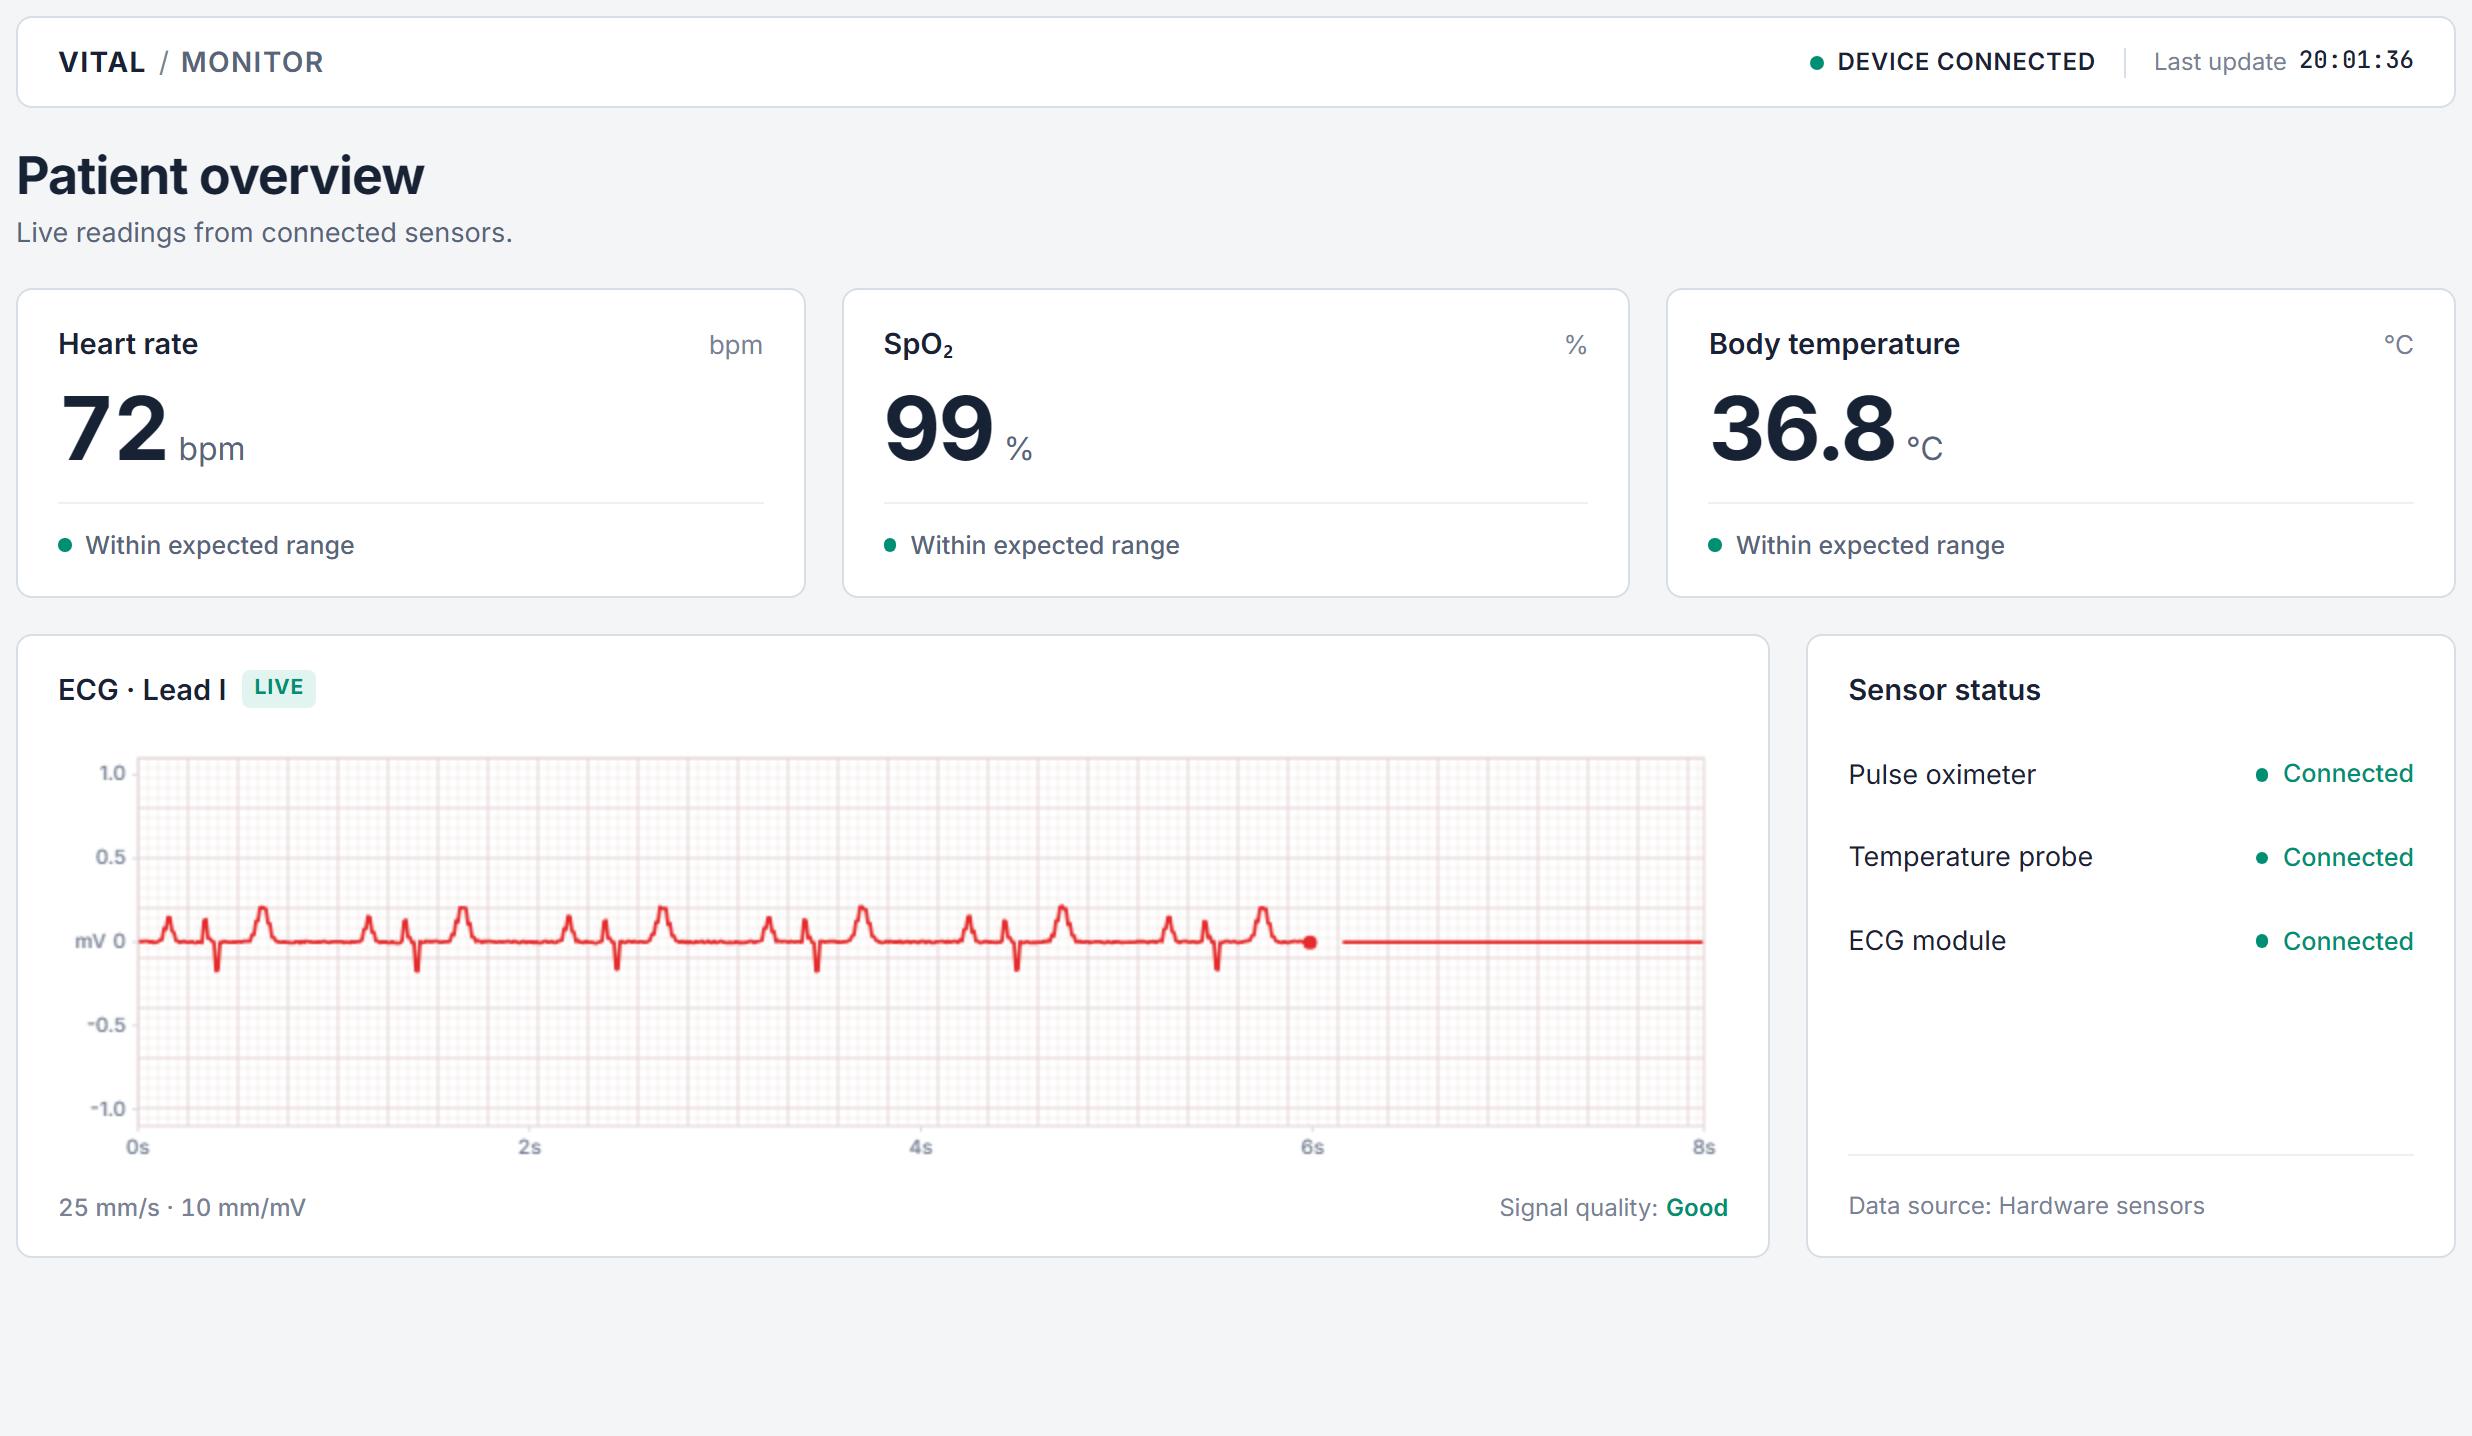
\includegraphics[width=\linewidth]{images/dashboard_live_telemetry.png}
\end{tcolorbox}
\vspace{-0.2cm}
\caption{Production Screenshot of the SmartHealth IoT Clinical React Telemetry Dashboard.}
\label{fig:dashboard_wireframe}
\end{figure}
\clearpage

% ==============================================================================
% PAGE 14: SECTION 8 — IMPLEMENTATION PLAN, MILESTONES AND TEAM RACI
% ==============================================================================
\section{Implementation Plan, Milestones and Team RACI}
\label{sec:implementation_plan}

\subsection{Eight-Week Implementation Roadmap and Critical Milestones}
The project follows an intensive 8-week execution plan (October -- November 2026). Hardware and backend pipelines develop concurrently during Weeks 1--2, merge into full-stack integration by Week 4, and reach the \textbf{MVP Checkpoint at Week 5} (Figure~\ref{fig:milestone_timeline}).

\vspace{0.08cm}
\begin{figure}[H]
\centering
\begin{tcolorbox}[tikzbox, title={Critical Milestone Progression Timeline (Weeks 1 to 8)}, left=4pt, right=4pt, top=3pt, bottom=3pt, width=\linewidth]
\centering
\resizebox{\linewidth}{!}{%
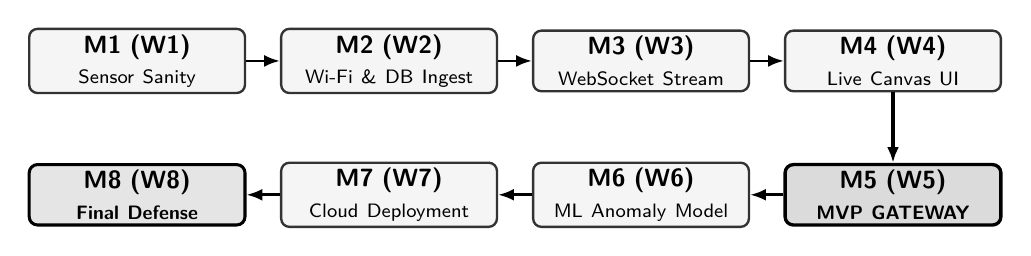
\begin{tikzpicture}[
    font=\sffamily\small,
    mstone/.style={rectangle, rounded corners=3pt, draw=black!80, fill=black!4, line width=0.85pt, align=center, text width=2.60cm, minimum height=0.74cm, inner sep=2pt},
    mvp/.style={rectangle, rounded corners=3pt, draw=black, fill=black!14, line width=1.2pt, align=center, text width=2.60cm, minimum height=0.74cm, inner sep=2pt},
    arr/.style={-{Latex[length=2.0mm, width=1.5mm]}, line width=0.95pt, color=black}
]

    % Row 1: Phase 1 — Weeks 1 to 4 (Left to Right)
    \node[mstone] (m1) at (-4.8, 0.85) {\textbf{M1 (W1)}\\\scriptsize Sensor Sanity};
    \node[mstone] (m2) at (-1.6, 0.85) {\textbf{M2 (W2)}\\\scriptsize Wi-Fi \& DB Ingest};
    \node[mstone] (m3) at (1.6, 0.85) {\textbf{M3 (W3)}\\\scriptsize WebSocket Stream};
    \node[mstone] (m4) at (4.8, 0.85) {\textbf{M4 (W4)}\\\scriptsize Live Canvas UI};
    
    % Row 2: Phase 2 — Weeks 5 to 8 (Right to Left return)
    \node[mvp] (m5) at (4.8, -0.85) {\textbf{M5 (W5)}\\\textbf{\scriptsize MVP GATEWAY}};
    \node[mstone] (m6) at (1.6, -0.85) {\textbf{M6 (W6)}\\\scriptsize ML Anomaly Model};
    \node[mstone] (m7) at (-1.6, -0.85) {\textbf{M7 (W7)}\\\scriptsize Cloud Deployment};
    \node[mstone, fill=black!10, draw=black, line width=1.1pt] (m8) at (-4.8, -0.85) {\textbf{M8 (W8)}\\\textbf{\scriptsize Final Defense}};

    % Row 1 Forward Connections
    \draw[arr] (m1) -- (m2);
    \draw[arr] (m2) -- (m3);
    \draw[arr] (m3) -- (m4);

    % Direct Downward Transition from Phase 1 to Phase 2 (Mid-Term Gateway)
    \draw[arr, line width=1.2pt] (m4.south) -- (m5.north);

    % Row 2 Return Connections
    \draw[arr] (m5) -- (m6);
    \draw[arr] (m6) -- (m7);
    \draw[arr] (m7) -- (m8);

\end{tikzpicture}%
}
\end{tcolorbox}
\vspace{-0.25cm}
\caption{Milestone Progression Timeline from Inception to Final Defense.}
\label{fig:milestone_timeline}
\end{figure}

\vspace{0.05cm}
\subsection{Team Roles, Responsibilities and RACI Governance Matrix}
Table~\ref{tab:raci_matrix} defines project task ownership across the five-member team using RACI (\textbf{R}esponsible, \textbf{A}ccountable, \textbf{C}onsulted, \textbf{I}nformed).

\vspace{0.06cm}
\begin{table}[H]
\centering
\footnotesize
\setlength{\tabcolsep}{4pt}
\renewcommand{\arraystretch}{1.08}
\setlength{\tblavail}{\dimexpr\linewidth - 12\tabcolsep - 7\arrayrulewidth\relax}
\setlength{\wA}{0.30\tblavail}
\setlength{\wB}{0.14\tblavail}
\setlength{\wC}{0.14\tblavail}
\setlength{\wD}{0.14\tblavail}
\setlength{\wE}{0.14\tblavail}
\begin{tabular}{|B{\wA}|C{\wB}|C{\wC}|C{\wD}|C{\wE}|C{0.14\tblavail}|}
    \hline
    \multicolumn{1}{|M{\wA}|}{\textbf{Functional Domain}} &
    \multicolumn{1}{M{\wB}|}{\textbf{Soumyajit}} &
    \multicolumn{1}{M{\wC}|}{\textbf{Bikkram}} &
    \multicolumn{1}{M{\wD}|}{\textbf{Debanjan}} &
    \multicolumn{1}{M{\wE}|}{\textbf{Biraj}} &
    \multicolumn{1}{M{0.14\tblavail}|}{\textbf{Sayan}} \\
    \hline
    Sensor Interfacing \& Circuits & A & \textbf{R} & C & I & I \\
    \hline
    ESP32 C++ Firmware \& Wi-Fi & \textbf{R} & C & C & I & I \\
    \hline
    FastAPI REST \& Validation & C & I & \textbf{R} & C & C \\
    \hline
    MongoDB Atlas Data Layer & I & I & \textbf{R} & I & C \\
    \hline
    WebSocket Distribution Engine & I & I & A & \textbf{R} & I \\
    \hline
    React UI \& Canvas ECG Plotter & C & I & C & \textbf{R} & I \\
    \hline
    ML Anomaly \& Trend Modeling & C & I & C & I & \textbf{R} \\
    \hline
    System Testing \& QA & A & C & R & C & \textbf{R} \\
    \hline
    Technical Report \& Presentation & A & R & R & \textbf{R} & R \\
    \hline
\end{tabular}
\caption{Team Task Allocation and RACI Governance Matrix.}
\label{tab:raci_matrix}
\end{table}
\clearpage

% ==============================================================================
% PAGE 15: RISKS, CONCLUSION & END OF REPORT
% ==============================================================================
\subsection{Engineering Risk Mitigation Matrix}
Table~\ref{tab:risk_matrix} highlights primary technical challenges and their engineering mitigations.

\vspace{0.06cm}
\begin{table}[H]
\centering
\footnotesize
\setlength{\tabcolsep}{4.5pt}
\renewcommand{\arraystretch}{1.03}
\setlength{\tblavail}{\dimexpr\linewidth - 6\tabcolsep - 4\arrayrulewidth\relax}
\setlength{\wA}{0.28\tblavail}
\setlength{\wB}{0.14\tblavail}
\setlength{\wC}{0.58\tblavail}
\begin{tabular}{|B{\wA}|C{\wB}|L{\wC}|}
    \hline
    \multicolumn{1}{|M{\wA}|}{\textbf{Technical Risk}} &
    \multicolumn{1}{M{\wB}|}{\textbf{Severity}} &
    \multicolumn{1}{M{\wC}|}{\textbf{Concrete Engineering Mitigation Strategy}} \\
    \hline
    AD8232 ECG Noise / 50\,Hz Hum & High & Power ESP32 via isolated 5V power bank (breaks mains ground loops); apply digital 50\,Hz notch and 0.5--40\,Hz bandpass filtering. \\
    \hline
    MAX30102 Ambient Light & Medium & Enclose sensor in an opaque velcro finger clip; use AC/DC ratio checks to reject motion-corrupted optical data. \\
    \hline
    I2C Bus Collision & High & Separate 7-bit addresses verified (\texttt{0x3C} OLED, \texttt{0x57} MAX30102); install $4.7\,\text{k}\Omega$ bus pull-ups; keep I2C transactions non-blocking. \\
    \hline
    Wi-Fi Telemetry Dropouts & Medium & Circular ring buffer in ESP32 RAM caches up to 10 seconds of vitals; auto-reconnect backoff prevents loop hangs. \\
    \hline
    High-Frequency Browser Lag & High & Batch ECG samples into 50-integer chunks (4 POSTs/sec); plot via HTML5 Canvas using GPU-accelerated \texttt{requestAnimationFrame}. \\
    \hline
    ML Schedule Delay (Fallback) & Low & Decoupled architecture: if ML training hits obstacles, FastAPI defaults anomaly flags to nominal; core IoT system runs independently. \\
    \hline
\end{tabular}
\caption{Technical Risk Assessment and Engineering Mitigation Matrix.}
\label{tab:risk_matrix}
\end{table}

\vspace{0.06cm}
\section{Conclusion and Future Scope}
\label{sec:conclusion}
The SmartHealth IoT system delivers a robust, accessible telemetry platform bridging embedded biomedical instrumentation and asynchronous cloud software. By capturing single-lead ECG, blood oxygen saturation, pulse rate, and temperature at the edge and streaming batched JSON payloads over Wi-Fi to a Python FastAPI backend, the system demonstrates reliable data ingestion, non-blocking cloud persistence in MongoDB Atlas, and low-latency anomaly estimation via an in-memory Isolation Forest model. Telemetry and live waveforms display smoothly on a modern React web dashboard via WebSockets.

\textbf{Future Engineering Roadmap:}
\begin{enumerate}[itemsep=1pt, parsep=0pt, topsep=1pt]
    \item \textbf{Custom PCB Fabrication:} Consolidate breadboard wiring into a compact 2-layer SMD PCB with isolated ground planes to suppress 50\,Hz noise.
    \item \textbf{BLE Hybrid Connectivity:} Add Bluetooth Low Energy (BLE) pairing for direct smartphone telemetry during outdoor mobility.
    \item \textbf{Edge TinyML Inference:} Port lightweight anomaly detection directly onto the ESP32 using TensorFlow Lite for Microcontrollers.
\end{enumerate}

\vspace{0.8cm}
\begin{center}
    \textbf{\large END OF REPORT}
\end{center}

\end{document}
